\documentclass{article}
\usepackage{graphicx}
\usepackage{amsmath}
\usepackage{amssymb}
\usepackage{setspace}
\usepackage{geometry}
 \geometry{
 a4paper,
 total={210mm,297mm},
 left=20mm,
 right=20mm,
 top=20mm,
 bottom=20mm,
 }


\begin{document}
\begin{center}
\begin{LARGE}
Further Notes on Equilibrium Subtraction and mode analysis for HBT-EP\\
\end{LARGE}
\begin{large}
\vspace{0.25 in}
Patrick Byrne \& Qian Peng\\
Columbia University Plasma Lab\\
Nov. 12 2014\\
\end{large}
\end{center}
\vspace{0.25 in}

\par
In the interest of increasing the amount of documentation regarding the various methods used in HBT-EP to analyze MHD fluctuations, and to extend the work of Chris Stoafer, this report will discuss how to properly isolate modes when sensors are broken, a method of extending the usefulness of polynomial subtraction by automatically finding the plasma-terminating disruption, how to take an m=0 subtraction when using the shaping coil, and how to determine the response of a plasma to an externally imposed error field (RMP).
%\begin{changemargin}{-2cm}{-2cm}
\vspace{0.25in}
\begin{center}
\begin{LARGE}
Isolating Modes with Incomplete Arrays
\end{LARGE}
\end{center}
\par
HBT-EP has several dead sensors.  The sensors that are broken have varied since the 2009 upgrade, as some have been repaired while others have failed.  A list is available on the wiki with the broken sensors, the last shot during which they were functioning and the first shot at which they began working again.  Please try to keep this list as up to date as possible, as analyzing data from bad sensors could potentially skew the results, as will be detailed below.
\par
This report will focus on a single HBT-EP shot, 84577. This shot presents significant challenges to analysis, since there is shaping, an RMP and half of the shells - and the sensors mounted to those shells - are retracted.  To begin with, we'll look only at the FBP3 (midplane top) sensors on the feedback sensor toroidal array.  Figure \ref{raw_sig} below shows those signals.
\par
\begin{figure}[h!]
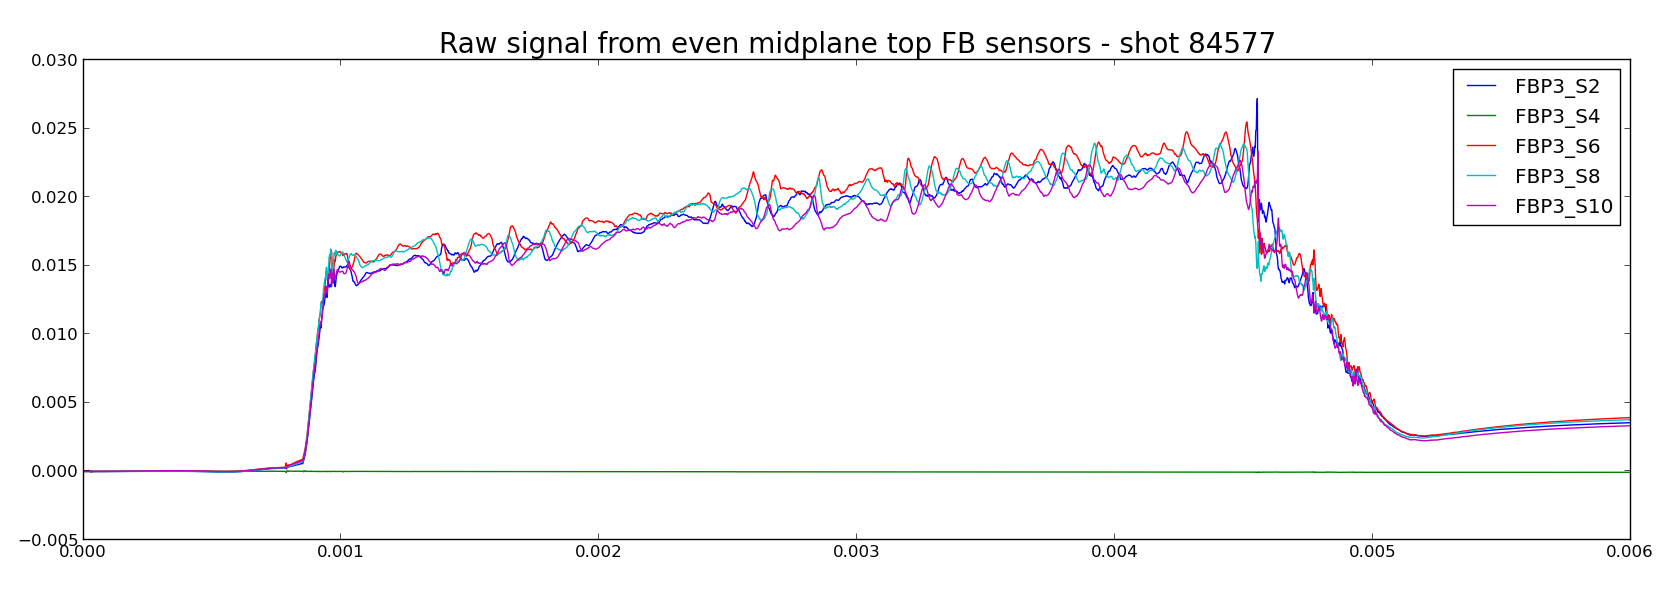
\includegraphics[width = \textwidth]{./Report_pic_raw_sig.png}\caption{Signal sets as extracted from tree}
\label{raw_sig}
\end{figure}
Instead of the usual set of 10 sensors on each toroidal array, we have only 5, due to retraction.  Furthermore, one of these 5 sensors is broken.  Obviously, an n=0 subtraction using all sensors would under-subtract by ~20\% the actual n=0 signal.   This is not disastrous, but it would leave an artifact which would then fall to the smoothing algorithm to resolve.  If you know that the sensor is dead ahead of time, of course, you can omit it from the averaging, and there will be no artifact at all.
\par
More subtle is the fact that averaging a sinusoidally varying function with non-evenly spaced observation points will not eliminate the higher order modes (n=1,n=2...) and this WILL interfere with our observations, in ways that polynomial smoothing will be unable to address, regardless of whether the dead sensor is included or excluded from the averaging.  See Figure \ref{n0_sig}\par
Takeaway:\\
\textbf{n/m = 0 subtractions on incomplete arrays introduce artifacts!!!}
\newpage
As you can see in Figure \ref{n0_sig}, with 4 of 5 signals - omitting the 'dead sensor' - being averaged, the fluctuating signal, while suppressed, is \textbf{not} completely eliminated.  In fact, since the artifact is being divided by 4 instead of 5, omitting the dead sensor exacerbates the problem! Subtracting this fluctuating signal as part of the equilibrium subtraction would be incorrect.  This has implications for boxcar smoothing, but in this report, I will focus solely on polynomial subtractions.
\begin{center}
\begin{figure}[h]
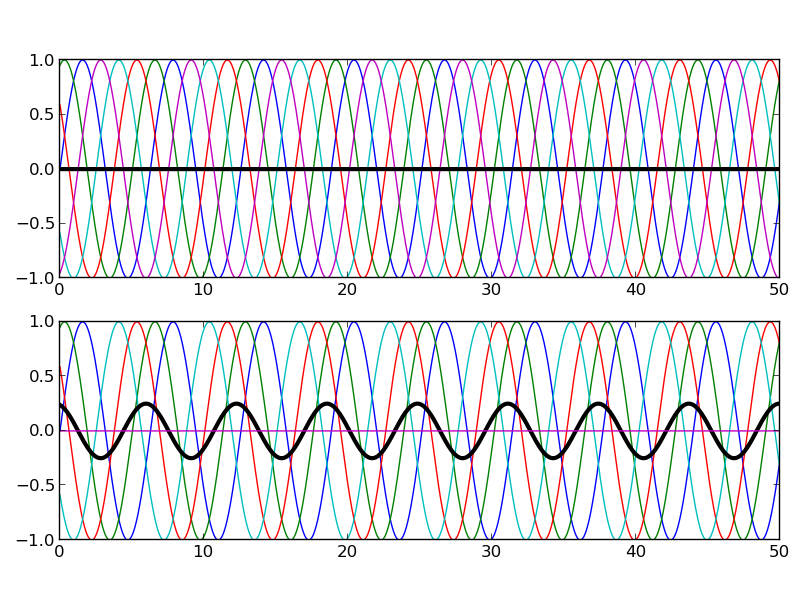
\includegraphics[width = \textwidth]{./Report_pic_minus_n0_sig.png}\caption{Two Signal sets - one complete and one missing a signal - and their 'n=0' average.  \newline
Dead sensor is excluded from the averaging in the lower plot}
\label{n0_sig}
\end{figure}
\end{center}
\par
I will skip the details of polynomial subtraction, as they were well covered in Chris's previous report, and only address the windowing issue he mentioned. Generally, the last vacuum bank to fire is the VF Electrolytic.  By pulling the value of VFE's trigger time from the tree, and choosing a reasonable padding (50us in this case) to get clear of any noise caused by the ignitrons firing, we can put a left edge on our analysis.\par
Finding the disruption is somewhat more difficult.  Though a full description is outside the scope of this paper, I use an algorithm that finds the minimum of $\frac{dI_p}{dt}$ to locate the current quench.  I then look for the minimum of $\frac{d^2I_p}{dt^2}$ in a time window stretching back 0.5ms from the current quench.  HBT-EP disruptions are characterized by a sharp,transient upward spike in $I_p$ just before the disruption and it is this sharply concave-down feature that we are looking for.  I find that the 'disruption time' given me by my code often corresponds quite well to the location of the actual disruption, although more work could be done to make it robust to non-standard disruptions.
\par
The main issue in smoothing is timescale.  Smoothing is easiest when the timescales in the experiment are widely separated.  I am using a 4th order mode, with a window that covers approximately 3ms.  Features that change slower than 333Hz are well subtracted, while faster features are left alone.  Our RMP has a 1kHz frequency, which is near enough 333Hz to cause concern, while the faster moving ~8kHz natural modes will be left largely unaffected.  Since we are most interested in the RMP, we ignore the time when the plasma would be reacting to it (2 - 3.2ms) when fitting the polynomial.  Figure \ref{poly_subtraction}. 
\begin{figure}[htb]
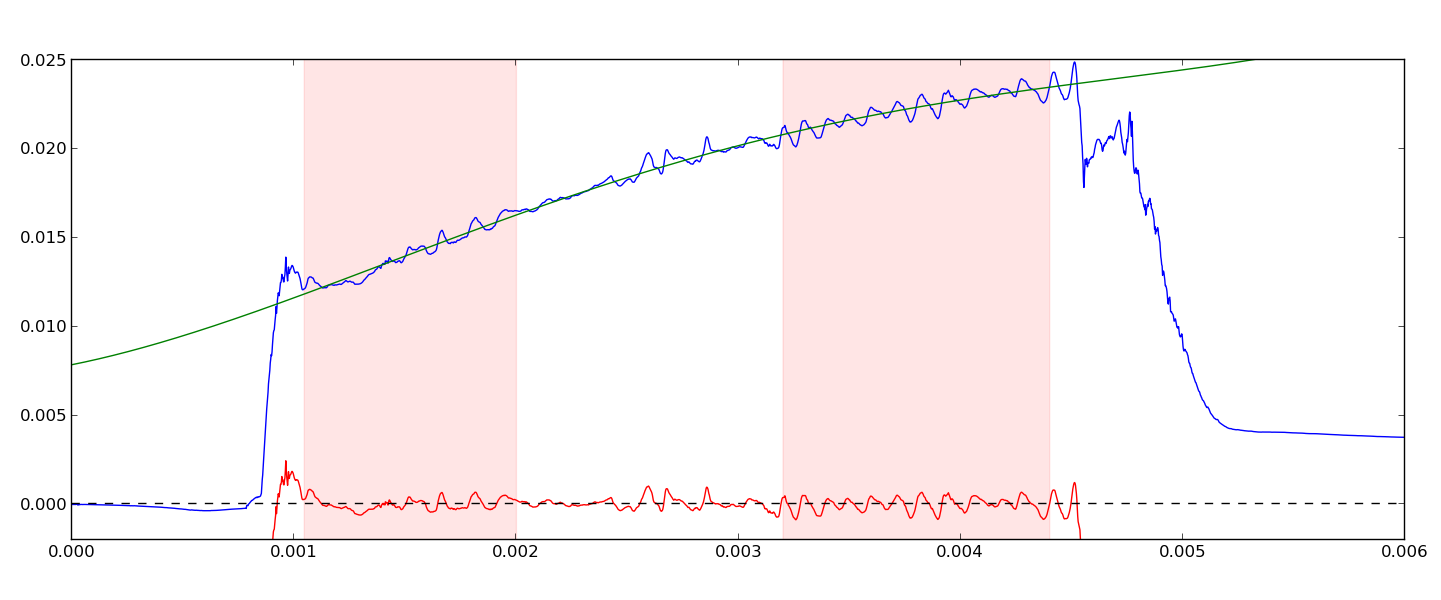
\includegraphics[width = \textwidth]{./Report_pic_minus_poly_sig.png}\caption{Sensor FB10P\_S3 signal, the polynomial fit (calculated using the red shaded range) and the signal after subtraction.}
\label{poly_subtraction}
\end{figure}
\par 
Extracting the fluctuations is done by applying an n=1 basis set to the fluctuations.  Again, this is trivial for a full sensor set, but in this case, care must be taken to avoid introducing artifacts.\par
One first constructs a Basis Matrix $\overrightarrow{B}$.  We will choose a Fourier basis, and since we will be looking at the n component of the mode, there are no issues with such a choice.  Each row of the set is the value of a particular sine or cosine basis *at the sensor angle*.  Since we are disregarding a dead sensor, there will be a jump between the values in B that correspond to the sensor angles on either side of the dead sensor.\par
We are solving an equation of the form:$$\begin{bmatrix}
a_1(t=0) & b_1(t=0) & \dots & b_n(t=0)\\
 & \vdots & \vdots & \\
a_1(t=t_f) & b_1(t=t_f) & \dots & b_n(t=t_f)
\end{bmatrix} \begin{bmatrix}
sin(\phi_0) & sin(\phi_2) &sin(\phi_3) & sin(\phi_4)\\
cos(\phi_0) & cos(\phi_2) &cos(\phi_3) & cos(\phi_4)\\
& \vdots & \vdots & \\
cos(n\phi_0) & cos(n\phi_2) &cos(n\phi_3) & cos(n\phi_4)
\end{bmatrix}$$
$$ = \begin{bmatrix}
sig(\phi_0,t=0) & sig(\phi_2,t =0) &sig(\phi_3, t =0) & sin(\phi_4, t = 0)\\
& \vdots & \vdots & \\
sig(\phi_0,t=t_f) & sig(\phi_2,t =t_f) &sig(\phi_3, t =t_f) & sin(\phi_4, t = t_f)
\end{bmatrix}$$
where $a_i$ and $b_i$ are the (time varying) amplitudes of the individual Fourier basis vectors, and the signal matrix $\overrightarrow{S}$ is simply the signal we get from the individual sensors.  We find the pseudoinverse of $\overrightarrow{B}$, $\overrightarrow{B^+}$,and solve for the amplitudes of the modes:

$$\overrightarrow{A(t)} = \overrightarrow{S}\overrightarrow{B^+}$$

The time varying magnitude of the mode is the quadrature sum of the individual pairs of amplitudes, and the phase of the modes are calculated using the arctangent.  With only 4 sensors, calculating more than one mode pair is not likely to give good results.\par
\begin{figure}[h]
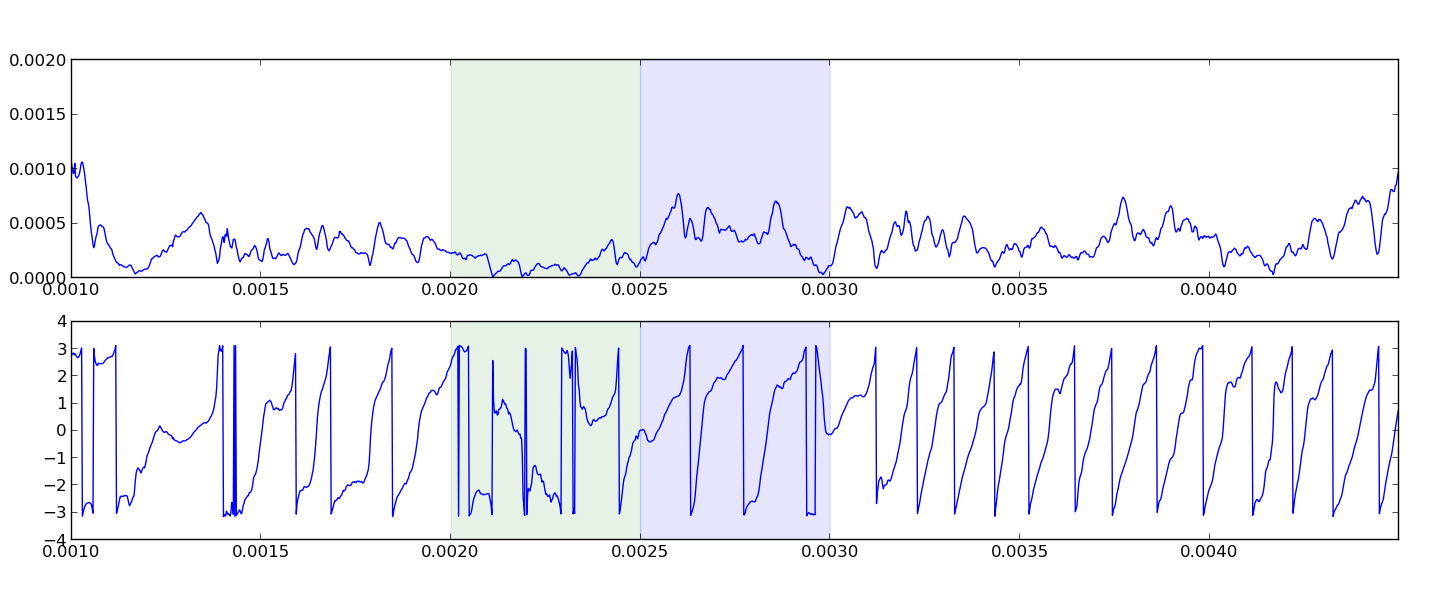
\includegraphics[width = \textwidth]{./Report_pic_n1_sig.png}\caption{Magnitude and phase of the reconstructed n = 1 mode.  Individual phases of the RMP flip are shaded.  Effect on mode phase is clear, magnitude is less so.}
\label{poly_sig}
\end{figure}
The results of performing this operation on the sensor signal, and reconstructing the n=1 signal is below.\\
This method is compared to a BD reconstruction during a window after the RMP but before the disruption.  Excellent tracking with phase is found, as well as good agreement in magnitude.  Both boxcar and polynomial smoothing were used for the bd analysis, and only minor differences in the magnitude time trace were found.  Since one of the main features that recommends the BD is its insensitivity to sensor errors, that such good agreement is found is very encouraging.
\newpage
\begin{figure}[htb]
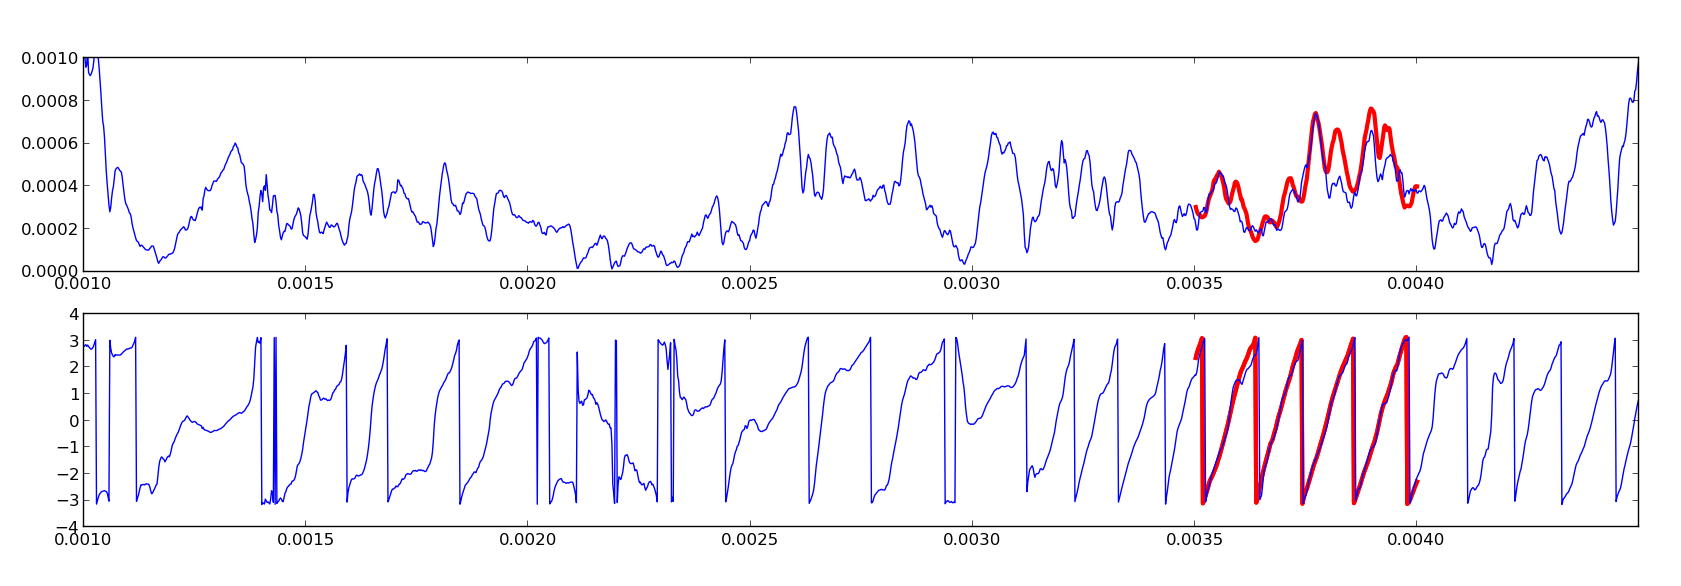
\includegraphics[width = \textwidth]{./Report_pic_bd_sig.png}\caption{The same magnitude and phase information with the BD results overplotted}
\label{bd_sig}
\end{figure}
\newpage
\begin{center}
\begin{LARGE}
Determining RMP Response
\end{LARGE}
\end{center}
\vspace{0.25in}
\par
One of HBT-EP's most important capabilities is the ability to probe the energetics of the MHD modes with RMP's of varying amplitude, shape, and/or rotation.  While most modes on HBT-EP grow and saturate on timescales faster than we can resolve, with the fairly reasonable assumption that unstable modes will grow larger in proportion to their $\delta$W's and that marginal modes will have the largest proportional response of all allows us to make determinations about the energetics of our modes, and their multimode characteristics.\par
Daisuke Shiraki performed an analysis of the response of HBT-EP plasmas to a variety of different mode shapes.  'Response' was calculated, in units of Gauss, as: $$ \frac{ \int^a_b{I_{rmp}B_{resp}dt}/\int^a_bdt }{ \sqrt{\int^a_b{I_{rmp}^2}/\int^a_bdt}}$$
As can be seen in Figure \ref{shiraki_RMP_shape}, the plasma responds most strongly to RMP's of helicity 3/1 and -4/1.
\begin{figure}[h!]
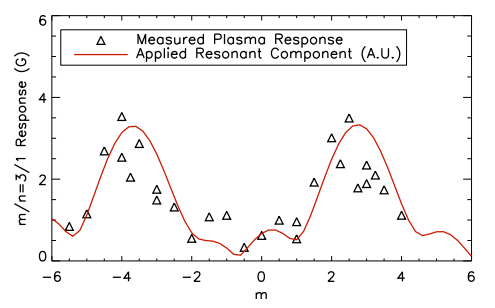
\includegraphics[width = \textwidth]{./Shiraki_thesis_Fig_7_1.png}\caption{Work done by Daisuke Shiraki, investigating circular plasma RMP response}
\label{shiraki_RMP_shape}
\end{figure}

\vspace{0.25in}
\begin{center}
\begin{LARGE}
Removing Shaping Pickup
\end{LARGE}
\end{center}
\par
The shaping coil introduces new challenges to equilibrium subtraction.  The other vacuum fields are spatially and temporally uniform, at least as compared to the shaping coil.  The shaping coil must be turned on after the plasma has formed, as the magnetic field null will be pushed out into the walls if the coil is on pre-breakdown.  This means that near the shaping coil, the equilibrium field will have a large, discontinuous phase that lasts for almost 1ms.  Combined with the foreshortening of the plasma lifetime caused by shaping, the notched subtraction method used for RMP analysis will not work, as there will not be enough stable, unchanging equilibrium on either side of the RMP for subtraction, see Figure \ref{PA_shaping}.\par
\begin{figure}[htb]
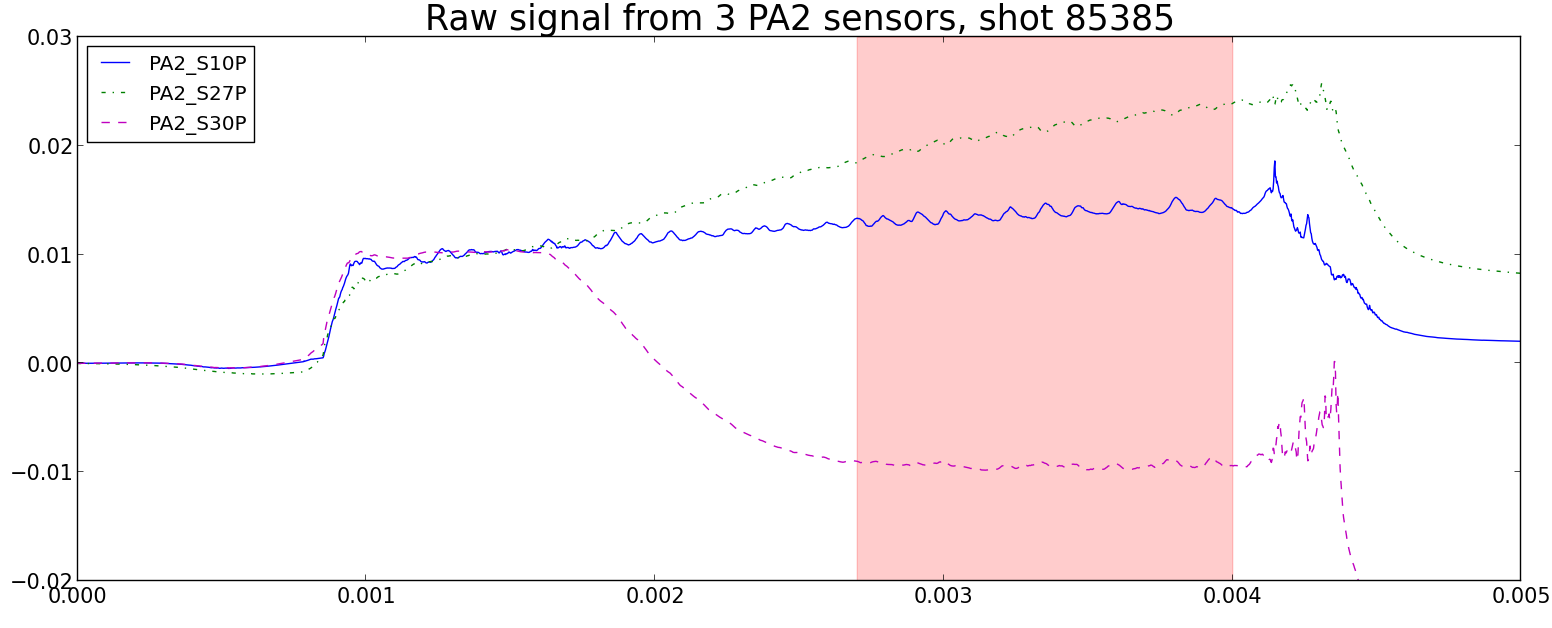
\includegraphics[width = \textwidth]{./shaping_raw_sig.png}\caption{The signal on various PA sensors during a shaped shot.  Useable polynomial smoothing regime is shaded, roughly 1ms}
\label{PA_shaping}
\end{figure}
HBT-EP has previously used a simple, constant multiplier based on a best fit subtraction for a given range of interest.  This is the easiest method, but leaves significant error left over.  When the shaping coil was installed, it became clear that this method would not be sufficient.\par
The method developed for subtraction of shaping coil pickup from the Ip and MR rogowskis, is a two-pole model including a linear multiplier, and two decaying exponentials that convolve with the time derivative of the vacuum coil's current.  While better in terms of reducing vacuum pickup to zero, this was done in a very ad-hoc way, with an unstable algorithm which was highly sensitive to initial guesses for the fit parameters.\par 
The newest method involves calculating a response function out of the Fourier transforms of both the current trace and the measured signal at the sensor.  By taking many shots, and then averaging the resultant response functions, we can subtract pickup with much greater fidelity, and with a much more robust and stable algorithm, than previously.  The process will be illustrated below.\par
The assumption used in this paper is that given a current in space, the field at any location is a function of the form:$$B = f(I)+f(\frac{dI}{dt})$$
or more explicitly: 
$$B = \alpha*I+\Sigma \int \beta_j*e^{\gamma_j*(\tau-t)} \frac{dI}{d\tau} d\tau$$
where the sum of convolutions represents the eddy currents that have been induced by the change in the current during the history of the shot.  This is a complicated function in the time domain, but taking advantage of the properties of the Fourier transform:$$F(B) = F(I)*(\alpha+\Sigma \beta_j*F(e^{\gamma_j(t)})*i*\omega)$$
We can derive a response function of the form:
$$H(\omega) = F(B)/F(I) = \alpha+i\omega*\Sigma( \beta_j*F(e^{\gamma_j(t)}))$$
Given the assumption of a rigid system, arbitrarily fine resolution, and perfect signal-to-noise ratio, this method should work perfectly for any arbitrary shot.  As we will see, the realities of HBT-EP causes this assumption to be less than perfect, but still quite good.
\par
Figure \ref{RF_subtraction_results} illustrates this.  3 sets of 6 shaping only vacuum shots were taken (shots 87697-87715).  5 of the shots in each set were taken, the Response Function of the PA2\_30P sensor to the shaping current was calculated, and averaged together.  This averaged response function is then used to predict the signal seen on the 6$^{th}$ shot of each set.  The subtraction is seen to be rather good, however there is a significant amount of noise on the rogowski, and convolving the PA signal with the rogowski returns a noisy prediction.  Noise on the SH rogowski can vary from runday to runday, so it should be possible to replicate this dataset when things are quieter.
\begin{figure}[htb]
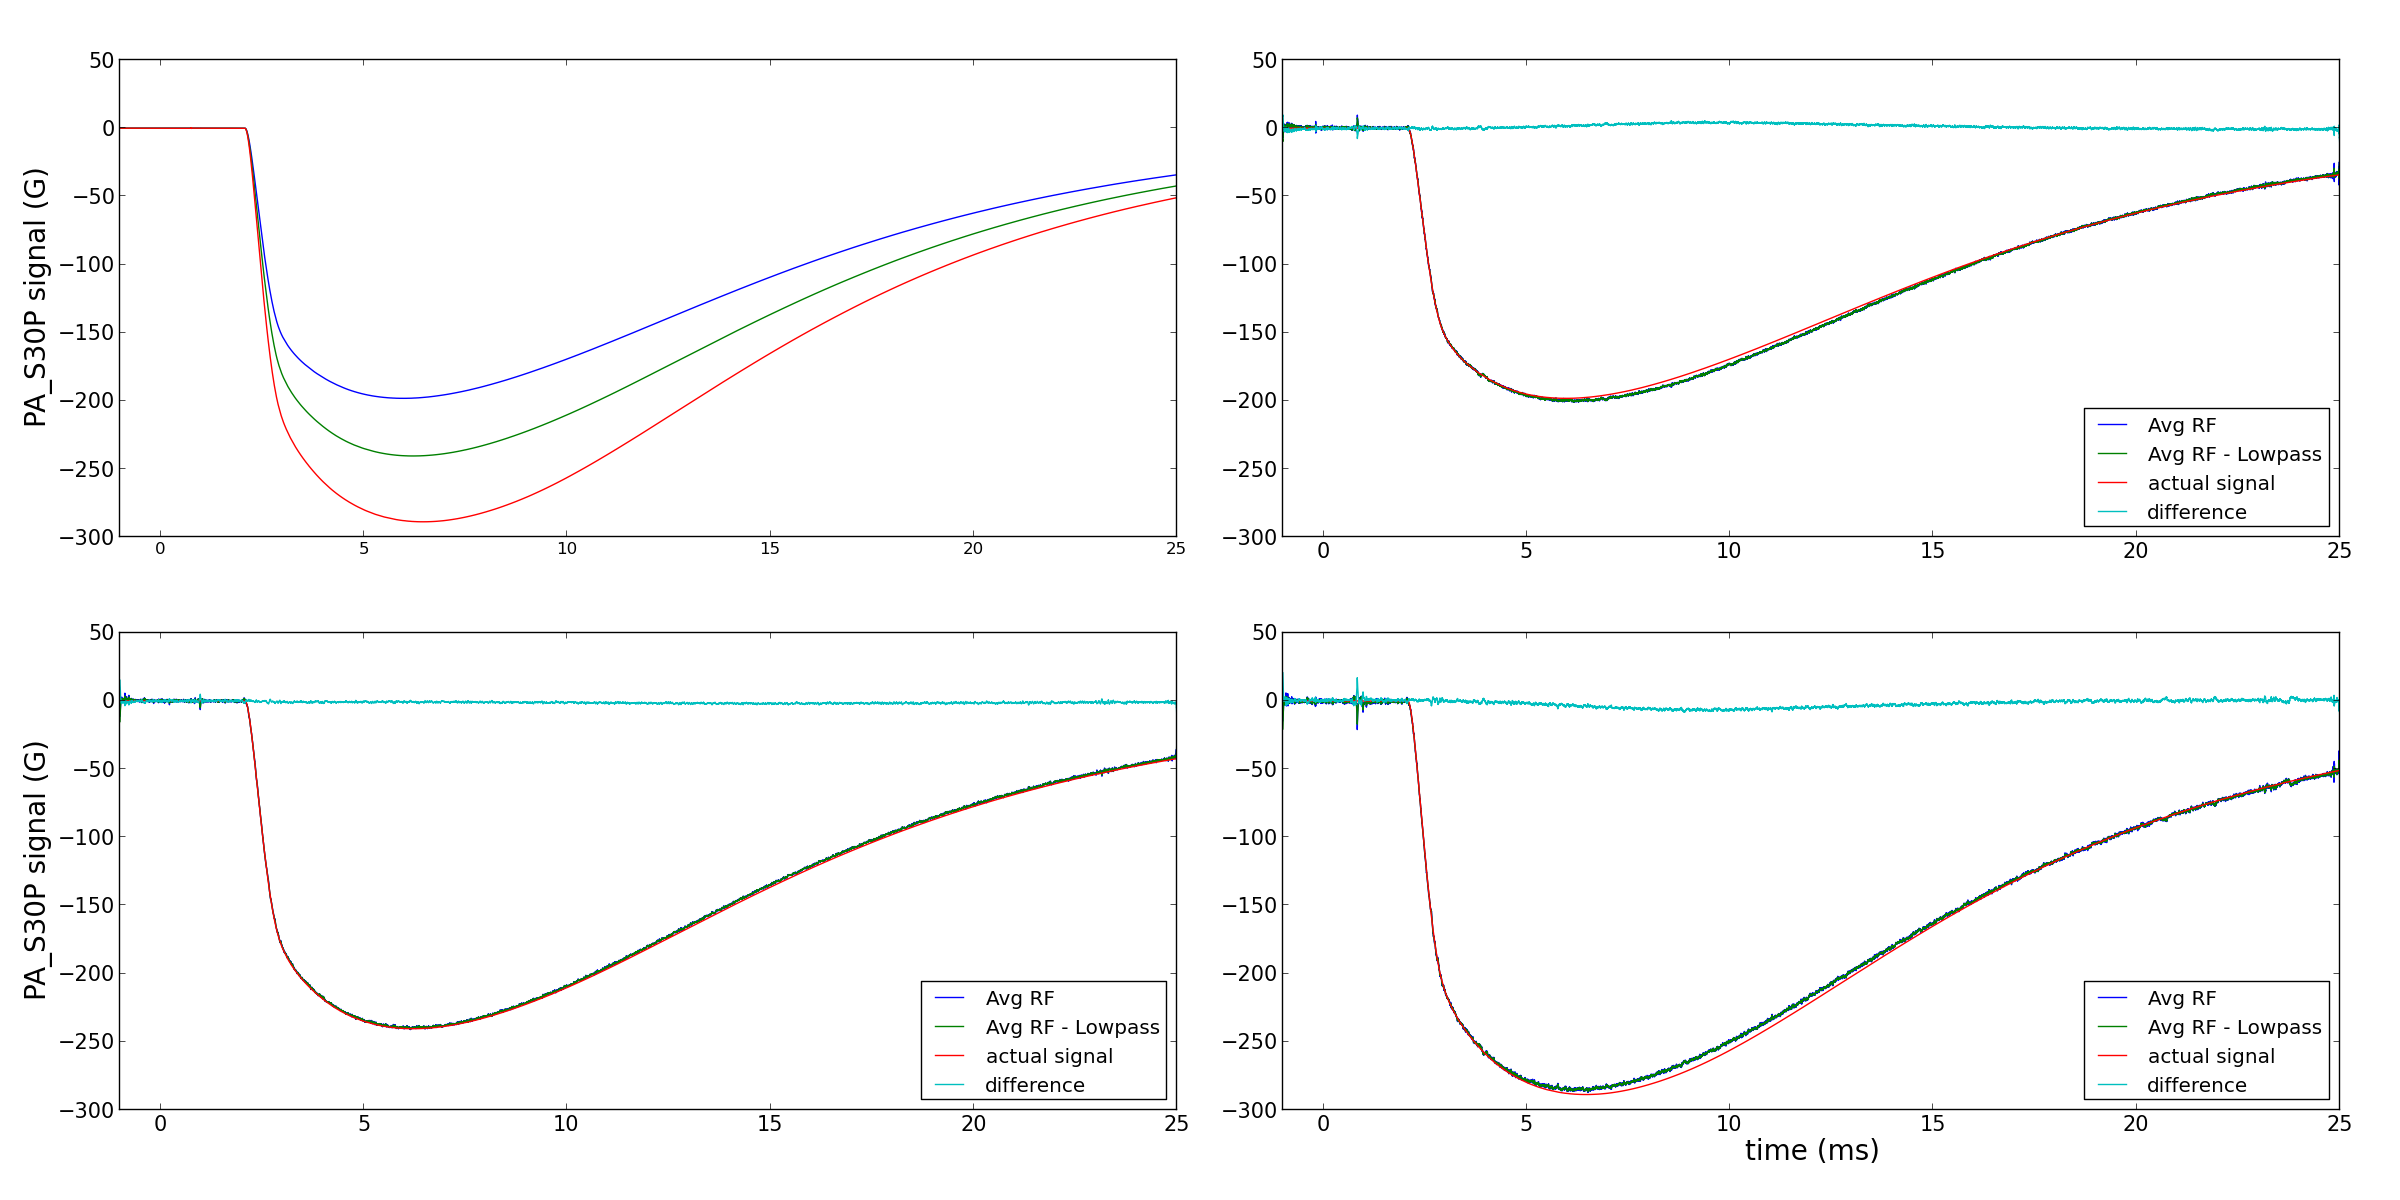
\includegraphics[width = \textwidth]{./RF_subtraction_results.png}\caption{Top left plot - PA2 sensor 30P pickup for three different shaping-only  shots.  Remaining three plots are one each of those shots, the predicted pickup, and the subtracted result}
\label{RF_subtraction_results}
\end{figure}
\par
\end{document}